\chapter{Basic Concepts} % (fold)
\label{cha:basic_concepts}
%
% * Contextualization
%     * Problems of augmented reality on the web
% * State of the art
%     * History of web ✔
%     * W3C ✔
%     * Browsers ✔
%         * The browser's high level structure ✔
%         * The browser's main functionality ✔
%     * HTML5
%     * JavaScript
%         * Language details ✔
%         * Typed arrays ✔
%         * requestAnimationFrame
%         * getUserMedia
%     * Canvas ✔
%     * Video ✔
%     * WebRTC ✔
%     * APIs ✔
%
\section{Web} % (fold)
\label{sec:basic_concepts:web}

Using concepts from existing hypertext systems, Tim Berners-Lee, computer scientist and at that time employee of CERN, wrote a proposal in March 1989 for what would eventually become the World Wide Web (WWW) \cite{WC2006}.

The World Wide Web is a shared information system operating on top of the Internet. Web browsers retrieve content and display from remote web servers using a stateless and anonymous protocol called HyperText Transfer Protocol (HTTP). Web pages are written using a simple language called HyperText Markup Language (HTML). They may be augmented with other technologies such as Cascading Style Sheets (CSS), which adds additional layout and style information to the page, and JavaScript (JS) language, which allows client-side computation. Browsers typically provide other useful features such as bookmarking, history, password management, and accessibility features to accommodate users with disabilities \cite{Grosskurth2005}.

In the beginning of the web, plain text and images were the most advanced features available on the browsers. In 1994, the World Wide Web Consortium (W3C) was founded to promote interoperability among web technologies. Companies behind web browser development together with the web community, were able to contribute to the W3C specifications \cite{WC2006}. Today's web is a result of the ongoing efforts of an open web community that helps define these technologies and ensure that they're supported in all web browsers. Those contributions transformed the web in a growing universe of interlinked pages and applications, with videos, photos, interactive content, 3D graphics processed by the Graphics Processing Unit (GPU), and other varieties of features without requiring any third-party plugins installation \cite{Hickson2013}. The significant reuse of open source components among different browsers and the emergence of extensive web standards have caused the browsers to exhibit ``convergent evolution'' \cite{Grosskurth2005}.

The browser main functionality is to present a web resource, by requesting it from the server and displaying it on the browser window. There are four major browsers used today: Internet Explorer, Firefox, Safari and Chrome. Currently, the usage share of Firefox, Safari and Chrome together is nearly 60\% \cite{Traffic2013}.

Three mature browser implementations were selected and, for each browser, a conceptual architecture was described based on domain knowledge and available documentation. Firefox version $16.0$, Safari version $6.0.4$ and Chrome version $25.0.1364$ were used to derive the reference architecture because they are mature systems, have reasonably large developer communities and user bases, provide good support for web standards, and are entirely open source.

The reference architecture for web browsers based on three well known open source implementations architecture, is shown in Figure \ref{figure:web_architecture}; It comprises eight major subsystems plus the dependencies between them:

\begin{enumerate}
  \item User interface: includes the address bar, back and forward buttons, bookmarking menu \etc\ Every part of the browser display except the main window where you see the requested resource.
  \item Browser engine: an embeddable component that provides a high-level interface for querying and manipulating the Rendering engine.
  \item Rendering engine: which performs parsing and layout for HTML documents, optionally styled with CSS.
  \item Networking subsystem: used for network calls, like HTTP requests. It has platform independent interface and underneath implementations for each platform.
  \item JavaScript parser: used to parse and execute the JavaScript code.
  \item XML Parser.
  \item UI backend: which provides drawing and windowing primitives, user interface widgets, and fonts. Underneath it uses the operating system user interface methods.
  \item Data persistence: which stores various data associated with the browsing session on disk, including bookmarks, cookies, and cache \cite{Grosskurth2005}.
\end{enumerate}

\begin{figure}[!htb]
  \centering
  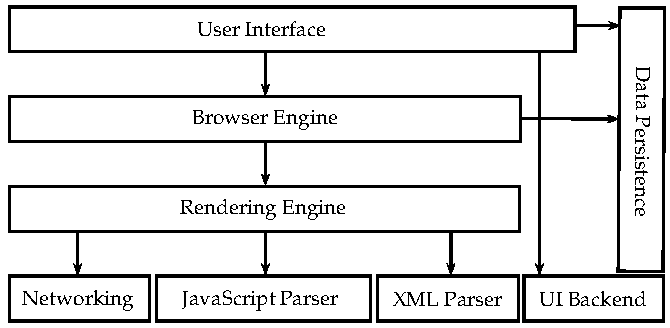
\includegraphics{chapters/basic_concepts/web_architecture.pdf}
  \caption{Reference architecture for web browsers}
  \label{figure:web_architecture}
\end{figure}

Browser subsystem are swappable and could vary for browser vendor, platform or operational system. The browsers mostly differ between different vendors in subsystems (2) the Browser engine, (3) the Rendering engine, and (5) the JavaScript parser. In Firefox, subsystems (2) and (3) are known as Gecko \cite{Firefox2013} \cite{Gecko2013}, Safari as WebKit \cite{Safari2013} \cite{WebKit2013} and Chrome uses a fork of WebKit project called Blink \cite{Chrome2010} \cite{Blink2013}. Those browsers subsystems, often called Browser engines, are shown on Figure \ref{figure:web_architecture_engines}.

Another common swappable subsystem is (5) the JavaScript parser. JavaScript is a lightweight, interpreted, object-oriented language with first-class functions, most known as the scripting language for Web pages \cite{Gecko2013}. The JavaScript standard is ECMAScript. As of 2013, all modern browsers fully support ECMAScript 5.1. Older browsers support at least ECMAScript 3 \cite{Gecko2013} \cite{International2009}.

\begin{figure}[!htb]
  \centering
  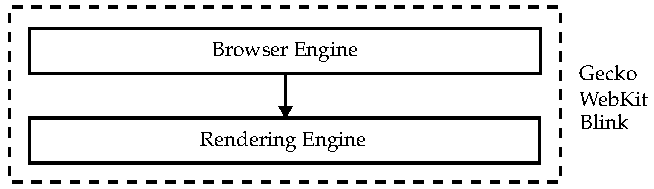
\includegraphics{chapters/basic_concepts/web_architecture_engines.pdf}
  \caption{Reference architecture for browsers engines}
  \label{figure:web_architecture_engines}
\end{figure}

The JavaScript language is intended to be used within some larger environment, be it a browser, server-side scripts, or similar. JavaScript core language features comprises few major features:

\begin{enumerate}
\item Functions and function scope: function is a subprogram that can be called by code external, functions have a scope it references for execution.
\item Global objects: refer to objects in the global scope, such as general-purpose constructors (\textit{Array, Boolean, Date} \etc), Typed array constructors (\textit{Float32Array, Int32Array, Uint32Array} \etc), Error constructors \etc.
\item Statements: consist of keywords used with the appropriate syntax (\textit{function, if...else, block, break, const, continue, debugger \etc}).
\item Operators and keywords: arithmetic operators, bitwise operators, assignment operators, comparison operators, logical operators, string operators, member operators, conditional operator \etc\ \cite{MDN2013}.
\end{enumerate}

As web applications become more and more powerful, adding features such as audio and video manipulation, access to raw data using WebSockets \cite{MDN2013}, and so forth, it has become clear that there are times when it would be helpful for JavaScript code to be able to quickly and easily manipulate raw binary data. In the past, this had to be simulated by treating the raw data as a string and using the \textit{charCodeAt()} method to read the bytes from the data buffer \cite{MDN2013} \cite{TypedArray2013}.

However, this is slow and error-prone, due to the need for multiple conversions, especially if the binary data is not actually byte-format data, but, for example, 32-bit integers or floats. Superior, and typed data structures were added to JavaScript specification, such as JavaScript typed arrays \cite{International2009}.

JavaScript typed arrays provide a mechanism for accessing raw binary data much more efficiently. This thesis takes advantage of typed arrays in order to achieve acceptable performance on the web of complex algorithms implementations.

A performance benchmark comparing regular \textit{vs} typed arrays were executed on the three well known open-source browsers, Firefox, Safari and Chrome. The comparison was executed on Mac OS X 10.8.3, 2.6 GHz Intel Core i7 16 GB 1600 MHz RAM. The array types selected were the not strongly typed \textit{Array}; \textit{Float32Array}, represents an array of 32-bit floating point numbers; \textit{Uint8Array}, represents an array of 8-bit unsigned integers.

For each array type a read and a write operation were executed $100,000$ times. In order to not compromise benchmark results caused by run-time type conversion \cite{International2009}, the write value used for each array type were proper selected, \eg\ \textit{Number} $1.0$ was used for regular arrays \textit{Array}, \textit{Number} $1.0$ was used for \textit{Float32Array}, and unsigned \textit{Number} $1$ for \textit{Uint8Array}. Regular \textit{vs} typed arrays performance benchmark is shown in Figure \ref{figure:typed_arrays_performance} \cite{TypedArrayPerformance2013}.

As conclusion, typed arrays provides faster read and write operations than regular arrays in JavaScript, \ie\ $7872$ \textit{ops/sec} for unsigned array \textit{vs} $4437$ \textit{ops/sec} for regular arrays in Firefox browser, similar behavior is noticeable on Safari and Chrome, thereby float and unsigned arrays are vastly used on complex algorithms implementations on the web.

\begin{figure}[!htb]
  \begin{tikzpicture}
      \begin{axis}[
          bar width=15pt,
          enlarge x limits=0.25,
          height= 200pt,
          legend cell align=left,
          scaled y ticks=false,
          symbolic x coords={Firefox,Safari,Chrome},
          width=0.85*\textwidth,
          xmajorgrids=true,
          xtick=data,
          ybar=\pgflinewidth,
          ylabel={Operations per second (ops/sec)},
          ylabel style={yshift=10pt},
          ymajorgrids=true,
          ymin=0
      ]
          \addplot[style={wblue, fill=wblue}]
              coordinates {
                (Firefox, 4437)
                (Safari, 2607)
                (Chrome, 679)
              };

          \addplot[style={wred, fill=wred}]
              coordinates {
                (Firefox, 5841)
                (Safari, 2797)
                (Chrome, 1510)
              };

          \addplot[style={worange, fill=worange}]
              coordinates {
                (Firefox, 7872)
                (Safari, 3089)
                (Chrome, 1510)
              };

          \legend{Array,Float32Array,Uint8Array}
      \end{axis}
  \end{tikzpicture}
  \caption{Regular \textit{vs} typed arrays performance benchmark}
  \label{figure:typed_arrays_performance}
\end{figure}

Nevertheless, reading and writing raw binary data using typed arrays only solves part of the problem of manipulating video and images data. The other missing feature was solved by HTML5 \cite{Hickson2013} \textit{canvas} element \cite{Canvas2013}, which one important feature is to provide access to the pixel matrix of those medias. The raw binary data is used by Augmented Reality (AR) algorithms.

The \textit{canvas} element \cite{Canvas2013} provides scripts with a resolution-dependent bitmap canvas, which can be used for rendering graphs, game graphics, art, or other visual images on the fly \cite{Canvas2013}. Authors should not use the \textit{canvas} element \cite{Canvas2013} in a document when a more suitable element is available, \eg\ it is inappropriate to use a \textit{canvas} element \cite{Canvas2013} to render a page heading. The usage of \textit{canvas} conveys essentially the same function or purpose as the canvas bitmap. Listing \ref{lst:canvas_element_markup} shows an example of a basic \textit{canvas} element \cite{Canvas2013} HTML markup given a width and height in pixels.

\begin{lstlisting}[language=HTML,label={lst:canvas_element_markup},caption=The HTML canvas element markup]
<canvas width="200" height="200"></canvas>
\end{lstlisting}

For each \textit{canvas} element \cite{Canvas2013} a ``context'' is available, then, from that, the drawing context can be accessed and JavaScript commands can be invoked to draw or read data. Browsers can implement multiple canvas contexts and the different APIs provide the drawing functionality. Most of the major browsers include the 2D canvas context capabilities. Individual vendors have experimented with their own three-dimensional canvas APIs \cite{Canvas2013}, but none of them have been standardized. The HTML5 \cite{Hickson2013} specification notes, ``A future version of this specification will probably define a 3D context'' \cite{Canvas2013}. Even though 3D context is not available in most part of the major browsers, three-dimensional applications are already being developed based on the 2D canvas context.

Is mandatory the use of the \textit{canvas} element \cite{Canvas2013} to develop AR applications on the web. Canvas provides APIs to: draw basic shapes, images, videos frames, Bezier and quadratic curves \cite{Hartley2004}; Apply transformations, translate, rotate and scale; Read raw pixel data \etc.

 The canvas \cite{Canvas2013} is a two-dimensional grid that could be described as a simple computer graphics coordinate system \cite{Hartley2004}. Normally $1$ unit in the grid corresponds to $1$ pixel on the canvas. The origin of this grid is positioned in the top left corner coordinate $(0,0)$. All elements are placed relative to this origin. So the position of the top left corner of the blue square becomes $x$ pixels from the left and $y$ pixels from the top coordinate $(x,y)$. The canvas coordinate space is shown on Figure \ref{figure:canvas_axis} \cite{MDN2013}.

 \begin{figure}[!htb]
   \centering
   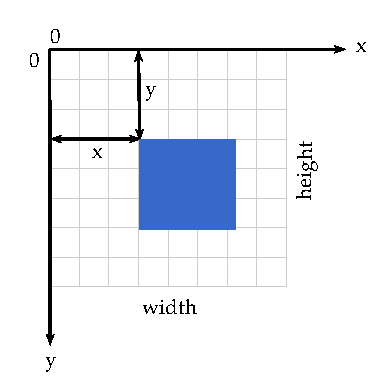
\includegraphics{chapters/basic_concepts/canvas_axis.pdf}
   \caption{The canvas coordinate space}
   \label{figure:canvas_axis}
 \end{figure}

 Videos and images pixels can be drew on a canvas bitmap. Canvas raw binary data can be accessed from the canvas \cite{Canvas2013} JavaScript API as an object of type \textit{ImageData} \cite{Canvas2013}. Each object has three properties: width, height and data. The data property is of type \textit{Uint8ClampedArray} that is a one-dimensional array containing the data in RGBA order, as integers in the range $0$ to $255$. The \textit{Uint8ClampedArray} interface type is specifically used in the definition of the canvas element's 2D API and its structure is  similar to the previous shown typed array \textit{Uint8Array} \cite{Canvas2013} \cite{TypedArray2013}.

The \textit{ImageData} data property, or array of pixels, is in row-major order, a multidimensional array in linear memory. For example, consider the 2×3 array $\begin{bmatrix}
1 & 2 & 3\\
5 & 5 & 6
\end{bmatrix}$, in row-major order it is laid out contiguously in linear memory as $\begin{bmatrix}
1 & 2 & 3 & 4 & 5 & 6
\end{bmatrix}$. Each array value is represented as integers between $0$ and $255$, where each four-integer group represents the four color channels of one pixel: red, green, blue and alpha (RGBA). While RGBA is sometimes described as a color space, it is actually simply a use of the RGB color model \cite{Gonzalez2007}. An example of the canvas \cite{Canvas2013} image data array of pixels is shown on Figure \ref{figure:imagedata_array}.

\begin{figure}[!htb]
  \centering
  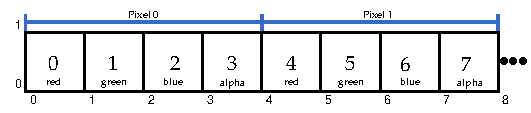
\includegraphics[width=\linewidth]{chapters/basic_concepts/imagedata_array.pdf}
  \caption{The canvas image data array of pixels}
  \label{figure:imagedata_array}
\end{figure}

Audio and video capture has been a limitation of web browsers for a long time. For many years the authors had to rely on browser plugins, such as Flash \cite{Flash2013} or Silverlight \cite{Silverlight2013} \cite{Rocks2013}. HTML5 \cite{Hickson2013} has brought a surge of access to device hardware, Geolocation (GPS), the Orientation API (accelerometer), WebGL \cite{WebGL2013} and the Real-time Communication Between Browsers specification (WebRTC) \cite{WebRTC2013} in conjunction with Media Capture and Streams specification, a set of JavaScript APIs that allow local media, including audio and video, to be requested from a platform trough \textit{getUserMedia} API \cite{WC2006}.

With \textit{getUserMedia}, the browser can access the camera and microphone input without a plugin. It's available directly into the browser. The access camera and microphone hardware access can be used in combination with the HTML5 \cite{Hickson2013} \textit{audio} and \textit{video} elements. The access flow of raw binary data captured from videos on modern browsers is shown on Figure \ref{figure:get_user_media} and comprises five major steps:

\begin{enumerate}
  \item  Hardware access: browser camera and microphone hardware is accessed \cite{WebRTC2013}.
  \item Streaming: hardware streams audio and video to the browser UI elements \cite{WebRTC2013}.
  \item UI elements: elements that displays the data stream, \eg\ \textit{audio} and \textit{video} elements \cite{Hickson2013}.
  \item Raw binary data: \textit{canvas} element \cite{Canvas2013} that ``hosts'' video frames providing access to the array of pixels.
\end{enumerate}

\begin{figure}[!htb]
  \centering
  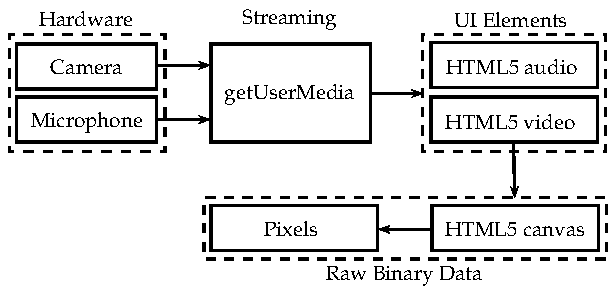
\includegraphics{chapters/basic_concepts/get_user_media.pdf}
  \caption{Access flow of raw binary data captured from videos on modern browsers}
  \label{figure:get_user_media}
\end{figure}

The \textit{audio} and \textit{video} elements is one of those HTML5 \cite{Hickson2013} features that gets a lot of attention. Often presented as an alternative to Flash \cite{Flash2013} in the media, the video element has advantages due to its natural integration with the other layers of the web development stack such as CSS and JavaScript as well as the other HTML elements. The three video formats supported by the three well known browsers cited in this thesis are, webm (VP8 Vorbis), mp4 (H.264 AAC) and ogv (Theora Vorbis) \cite{WC2006} \cite{Rocks2013}. The audio formats available are ogg (Theora Vorbis) and mp4 (H.264 AAC). An example of \textit{getUserMedia} API being used to capture the camera and microphone using a \textit{video} element to display is shown on Listing \ref{lst:get_user_media}.

\begin{lstlisting}[language=C++,label={lst:get_user_media},caption=Capture and display microphone and camera]
<video autoplay></video>
<script>
  var video = document.querySelector('video');
  navigator.getUserMedia(
    {video: true, audio: true},
    function(localMediaStream) {
        video.src = window.URL.createObjectURL(localMediaStream);
        video.onloadedmetadata = function(e) {
          // Ready to go.
        };
    },
    onFail);
</script>
\end{lstlisting}

% section web (end)

\section{Augmented Reality} % (fold)
\label{sec:basic_concepts:augmented_reality}

Imagine a technology in which you could see more than others see, hear more than others hear, and even touch things that others cannot. A technology able to perceive computational elements and objects within our real world experience that help us in our daily activities, while interacting almost unconsciously through mere gestures and speech.

With such technology, mechanics could see instructions what to do next when repairing an unknown piece of equipment, surgeons could take advantage of augmented reality while performing surgery on them and we could read reviews for each restaurant in the street we're walking in on the way to work \cite{Krevelen2010}.

Augmented reality (AR) is this technology to create a ``next generation, reality-based interface'' \cite{Krevelen2010} and is moving from laboratories around the world into various industries and consumer markets. AR supplements the real world with virtual (computer-generated) objects that appear to coexist in the same space as the real world. AR was recognized as an emerging technology of 2007 \cite{Krevelen2010}, and with today's smart-phones and AR browsers we are starting to embrace this very new and exciting kind of human-computer interaction. Three important aspects of an AR system \cite{Benford1998}:

\begin{enumerate}
  \item Combines real and virtual objects in a real environment.
  \item Aligns real and virtual objects with each other.
  \item Runs interactively, in three dimensions, and in real time.
\end{enumerate}

On the reality-virtuality \textit{continuum} by Milgram and Ki \cite{Mistry2009}, Augmented Reality (AR) is one part of the general area of mixed reality. Both virtual environments (or virtual reality) and augmented virtuality, in which real objects are added to virtual ones, replace the surrounding environment by a virtual one. In contrast, AR provides local virtuality. The reality-virtuality \textit{continuum} is shown on Figure \ref{figure:reality_continuum}.

\begin{figure}[!htb]
  \centering
  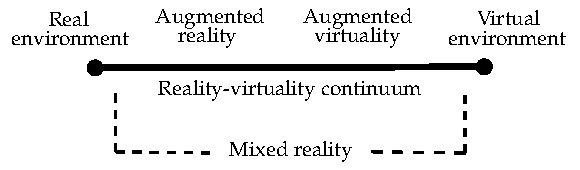
\includegraphics{chapters/basic_concepts/reality_continuum.pdf}
  \caption{Reality-virtuality continuum}
  \label{figure:reality_continuum}
\end{figure}

The first AR prototypes, shown in Figure \ref{figure:first_head_mount}, created by computer graphics pioneer Ivan Sutherland and his students at Harvard University and the University of Utah, appeared in the 1960s and used a see-through to present 3D graphics \cite{Benford1998}. It took until the early 1990s before the term ``augmented reality'' was proposed by Caudell and Mizell \cite{Benford1998}, scientists at Boeing Corporation who were developing an experimental AR system to help workers put together wiring harnesses.

\begin{figure}[!htb]
  \centering
  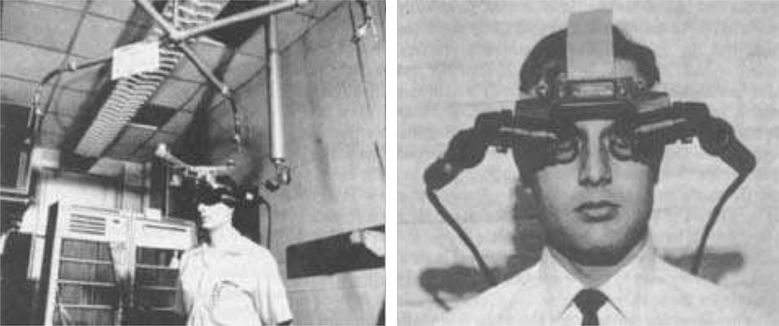
\includegraphics[width=\linewidth]{chapters/basic_concepts/first_head_mount.png}
  \caption{The world's first head-mounted display with the ``Sword of Damocles''}
  \label{figure:first_head_mount}
\end{figure}

By the late 1990s, as AR became a distinct field of research. Displays, trackers, graphics computers and software remain essential in many AR experiences. There are several displays devices that could be used on AR applications, the major ones could be divided as follows \cite{Benford1998}:

\begin{enumerate}
  \item Visual display: video see-through, optical see-through and projective.Video see-through is the closest to virtual reality, where the virtual environment is replaced by a video feed of reality and the AR is placed on the video frames. The optical see-through systems combine computer-generated imagery with holographic optical elements (HOEs), providing a ``through the glasses'' image of the real world. The last sub-category in section (1) is the projective, these displays have the advantage that they do not require special eye-wear, it projects the information into a surface, wall or even the human palm \cite{Benford1998}. The use of a regular computer monitor has become popular as a visual display since AR techniques are now available on the Internet.
  \item Display positioning: head-worn, hand-held and spatial. Head-worn is a visual displays attached to the head include the video or optical see-through head-mounted display (HMD), virtual retinal display (VRD), and head-mounted projective display (HMPD). Google Inc. released a first-class optical HDM called Project Glass shown on Figure \ref{figure:google_glass} \cite{Glass2013}. The hand-held sub-category includes hand-held video or optical see-through displays as well as hand-held projectors, it is currently the best choice to introduce AR to a mass market due to low production costs and ease of use since it may be based on existing consumer products, such as mobile phones. The last sub-category in section (2) is the spatial, those are displays that could placed statically within the environment and include screen-based video see-through displays \cite{Benford1998}.
\end{enumerate}

\begin{figure}[!htb]
  \centering
  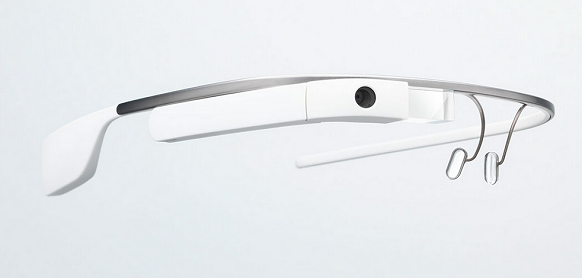
\includegraphics[width=\linewidth]{chapters/basic_concepts/google_glass.png}
  \caption{Optical head-mounted display Google Glass \cite{Glass2013}}
  \label{figure:google_glass}
\end{figure}

In this thesis, it was designed and implemented an Augmented Reality (AR) framework aiming to provide a common infrastructure to develop applications and to accelerate the use of those techniques on the web in commercial products. It runs on native web browsers without requiring third-party plugins installation, therefore any browser ready device can eventually use the proposed cross-platform code base to develop AR applications. In order to develop for different devices different skills are required, since APIs and programming languages may differ between them. In the current day, the most popular devices, such as smart phones, tablets, computers, notebooks and HDM (\ie\ Google Glass) are browser ready. They all could benefit from a reusable, cross-platform framework for AR applications.

% section augmented_reality (end)

\section{Augmented Reality on the Web} % (fold)
\label{sec:basic_concepts:augmented_reality_on_the_web}

Client-side native web applications use to have intrinsic performance limitations, although this premise is changing. Browsers are evolving very fast when compared to the the previous decade. JavaScript language wasn't prepared to handle typed data structures able to manipulate raw binary data safely, all the computational complexity required by AR algorithms was too much for that growing environment. Browsers weren't able to capture audio and video natively, without plugin installation, an essential feature for AR applications. This reality has changed, this involves the use of several modern browser specifications as well as implementation of different computer vision algorithms and techniques into the browser environment taking advantage of all those modern APIs. Some optimizations are discussed and implemented on this work in order to achieve good results when compared with similar implementations in compiled languages.

% section augmented_reality_on_the_web (end)

\section{Tracking} % (fold)
\label{sec:basic_concepts:augmented_reality_tracking}

Tracking an object in a video sequence means continuously identifying its location when either the object or the camera are moving. There are a variety of approaches, depending on the type of object, the degrees of freedom of the object and the camera, and the target application.
2D tracking typically aims at following the image projection of objects or parts of objects whose 3D displacement results in a motion that can be modeled as a 2D transformation \cite{Lepetit2005}.

One of the major responsibility of a tracking algorithms is to extract information that allows superposing computer generated images on real scenes. Many potential Augmented Reality (AR) applications have been explored, such as medical visualization, maintenance and repair, annotation, entertainment, aircraft navigation and targeting. The objects in the real and virtual worlds must be properly aligned and the system latency should also be low, lest the illusion that the two worlds coexist be compromised. \cite{Lepetit2005} Due to the importance of tracking in AR, this area owns the biggest number of publications and challenge requests on the International Symposium on Mixed and Augmented Reality (ISMAR) \cite{Zhou2008}.

There are a variety of ways to track a real environment: \eg\ global positioning system (GPS), mechanical trackers, magnetic trackers, ultrasonic trackers \etc\ \cite{Krevelen2010}, but they all have their weaknesses. Mechanical trackers are accurate enough, although they tether the user to a limited working. Magnetic trackers are vulnerable to distortions by metal in the environment. Ultrasonic trackers suffer from noise and tend to be inaccurate at long ranges because of variations in the ambient temperature \cite{Lepetit2005}.

By contrast, vision has the potential to yield non-invasive, accurate and low-cost solutions to this problem, provided that one is willing to invest the effort required to develop sufficiently robust algorithms. Bringing video tracking based techniques on the web are the focus of this work \cite{Lepetit2005}.

In some cases, it is acceptable to add fiducials, such as special markers, to the scene or target object. The addition of fiducials in the scene, also called landmarks or markers, greatly helps since they constitute image features easy to extract, and they provide reliable, easy to exploit measurements for the pose estimation.

It is therefore much more desirable to rely on naturally present features, such as edges, corners, or texture. The latter, makes tracking far more difficult because finding and following feature points or edges can be difficult. There are too few of them on many typical objects. Section \ref{sec:basic_concepts:markerless_tracking_technique} details markerless tracking techniques, main technique implemented on the web by this thesis.

% section augmented_reality_tracking (end)

\section{Markerless Tracking Techniques} % (fold)
\label{sec:basic_concepts:markerless_tracking_technique}

Markerless Augmented Reality (MAR) systems integrate virtual objects into a real environment in real-time, enhancing user's perception of and interaction with the world. This approach is not based on the use of traditional artificial markers that need to be placed in the world to be tracked by the system in order to calculate their position and orientation \cite{Teichrieb2007}, instead, MAR relies on naturally present features in order to position virtual objects. Tracking techniques become more complex in MAR systems when compared to marker techniques.

MAR can be classified in two major types: Model based and Structure from Motion (SfM) based. The online monocular MAR taxonomy is shown on Figure \ref{figure:mar_taxonomy}.

\begin{figure}[!htb]
  \centering
  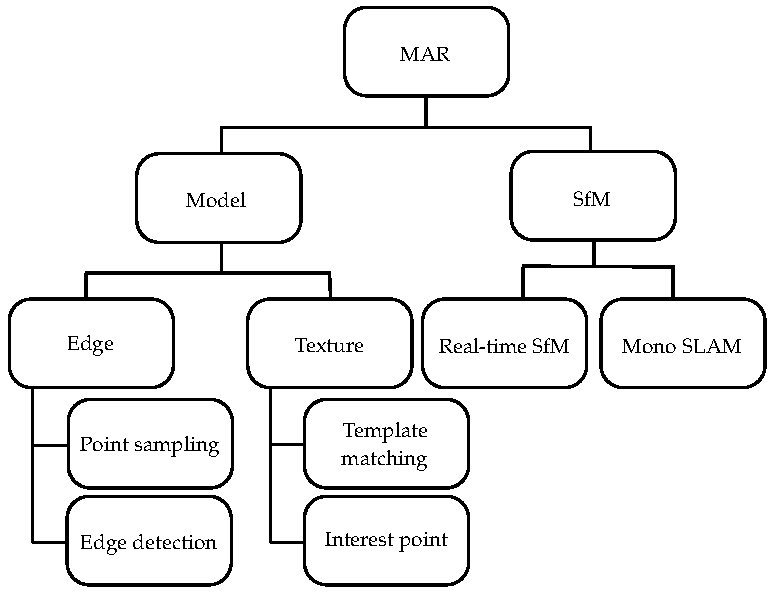
\includegraphics{chapters/basic_concepts/mar_taxonomy.pdf}
  \caption{Online monocular Markerless Augmented Reality taxonomy}
  \label{figure:mar_taxonomy}
\end{figure}

\subsection{Structure from Motion (SfM)} % (fold)
\label{sub:basic_concepts:markerless_tracking_technique:sfm}

SfM based systems have advantages, since they are capable of continuously tracking the camera in unknown scenes, although it's not detailed in this thesis. Model based systems usually requires lower computational complexity, ideal to the web environment.

% subsection sfm (end)

\subsection{Model Based} % (fold)
\label{sub:basic_concepts:markerless_tracking_technique:model_based}

The advantage of using a model based approach is the possibility of interaction between real and virtual worlds, like occlusion and collision. In order to accomplish such types of interaction, the application exploits the fact that the real object pose is known and its structure is described by the 3D model. Model based approaches require an a priori knowledge about the real scene. Due to the offline model acquiring process, these techniques are, in general, not totally online and cannot be used in unprepared environments. Furthermore, tracker initialization is usually done manually or requires a prior training in order to be automatic \cite{Teichrieb2007}. Model based techniques can be classified in three categories:

\begin{enumerate}
  \item Edge based: the camera pose is estimated by matching a wireframe 3D model of an object with the real world image edge information.
  \item Optical flow based: rely on spatial information obtained by image-model matching extracted from the relative movement of the object projection onto the image.
  \item Texture based: takes into account texture information presented in images.
\end{enumerate}

The technique implemented in this thesis is based on texture, therefore a much detailed description is presented in the following lines. Texture based could be divided into two sub-categories: template-matching and interest point.

The template matching approach is based on global information, this subcategory lies in its ability to treat complex patterns that would be difficult to model by local features. These techniques are also called sum-of-square-difference (SSD), as they consist in minimizing the difference between a region of the image and a reference template.

The subcategory of interest point based (or feature points) techniques takes into account localized features. As a result, this subcategory is less computer-intensive than template matching approach, this characteristic makes interest point technique a good choice for AR applications on the web.

The tracking solution proposed, uses Features from Accelerated Segment Test (FAST) \cite{Rosten2010} to extracts feature points using corner detection. This technique is detailed on Section \ref{sec:ar_library_for_the_web:interest_point_detection}. Binary Robust Independent Elementary Features (BRIEF) \cite{Calonder2010} is used as an efficient feature point descriptor (also known as feature matching), detailed on Section \ref{sec:ar_library_for_the_web:interest_point_matching}. Both techniques combined results in a high performance marker-less tracking solution which fits the native web needs due to the existing browsers performance limitations.

% subsection basic_concepts:markerless_tracking_technique:model_based (end)

% section markerless_tracking_technique (end)

% chapter basic_concepts (end)